% Each line that start by a '%' is a comment, it means, you can put all the shit in the world you want here,  
% Latex will not "interpret" it (eg. it does not transform it as text in the final PDF).

% The next line defines that this will be an article, it changes the "shape" of the document.
% There is different "class" available (article, book, report...), try it! 
\documentclass{article}    % comment this line if you uncomment the next line
% \documentclass{report}   % uncomment this line (only remove the '%' in the begining of the line)

\usepackage{graphicx}  % This line includes "packages". 
% Each package give access to new elements that you can use in your document.
% Here, graphicx gives access to stuffs related the handling of images, but I don't remember exactly what...
\usepackage{url} % This package is to get access to \url{}, it should work out of the box

\begin{document} % this is the beginning of the document per say

\title{Introducion a \LaTeX{} para la Patrona Hermosa}
\author{Pollito el Patron}
 
\maketitle  % this build the title using information from above (arriba?)

% As a rule, whenever there is a \begin{stuff} a \end{stuff} is required and everything in between
% is part of "stuff"
\begin{abstract} % This is the beginning of the abstract if you need one
The abstract text goes here.
In this document, we will briefly see how to include graphics and equations in your latex document.
Please note that this document is only dedicated to a special patrona!
\end{abstract}

\section{Expressions \& Figures}

\subsection{Expressions}
Oye Patrona, aqui hay expressiones, mira en el codigo como puedes escribirlos!
Here is some examples about how you can write them.
You can see with the equation~\ref{simple_equation}, that it is displayed with a number you can reference and it is positioned in the center of the document.

\begin{equation}
    \label{simple_equation}  % this label is used to reference the equation with \ref{} in your text
    \alpha = \sqrt{ \beta }
\end{equation}

This one cannot be referenced, but is displayed in the center again. 
It requires that the code is set in between special characters (look in the code) and on a new line with an empty line before and after.

\[\int ^{a}_{b}f\left( a\right)\]

Finally, if you want to write an equation inside of a sentence, you need to use others (almost as before), but you just put them as \(x^{a b c}\) in the sentence.

\noindent To help you write equations, you can use this website (\url{https://webdemo.myscript.com/views/math/index.html#}).
It let you draw your equations with the mouse (or the finger I guess on your phone?) and write the \LaTeX{} equivalent that you can copy/paste in your document.
It's hard to write with the mouse... but it works well! 
Be careful, when you copy/paste a formula, you need to put in a good "environement", i.e, in between begin/end tags or in between special characters.
If you need, there is also this website that can help you: \url{https://www.latex4technics.com/}, if you have problem editing or finding symbols.

\subsection{Figures}
We will see now how to insert a picture.
It's easier in the sense that even there is way of doing it, usually, one is enough. Again, you can reference figure~\ref{tryingsohard} using the label as for the equation.
There is more details in the code directly patrona!

\begin{figure}[htb] % the stuffs in between [] indicates the preferred positions when the image is included 
% 'h' means "here", 't' means "top" of page, and 'b' means "bottom" of page. The '!' is to force those positions, but you can remove it if you don't like it.
    \centering
    % you put here the name of the file with the picture
    % the line "width=0.8\linewidth" means that the picture width must be 0.8 times the with of a line
    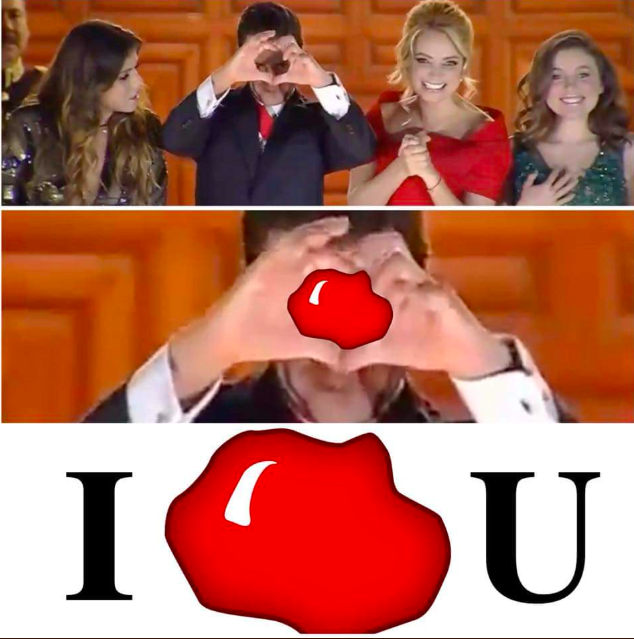
\includegraphics[width=0.8\linewidth]{myfigure}  
    \caption{Trying so hard}
    \label{tryingsohard}
\end{figure}

\section{Conclusion}
Writing \LaTeX{} requires a little bit of practicing, but you can do it Patrona!
I really hope this helped you.
I wrote it with you in mind and I enjoyed each moment of it.

\end{document}  % This marks the end of the document. As a rule, whenever there is a \begin{stuff} a \end{stuff} is required 